\documentclass[a4paper, 12pt]{report}

\usepackage[utf8]{inputenc} 	% accents
\usepackage[T1]{fontenc}      	% caractères français
\usepackage{graphicx}		% images

\title{Projet INFO-H-303 : Villo!}
\author{Hereman Nicolas, Van Brande Rodrigue}
\date{24 avril 2015}

\begin{document}
\maketitle 

\section*{Diagramme entité-association} % Diagramme
	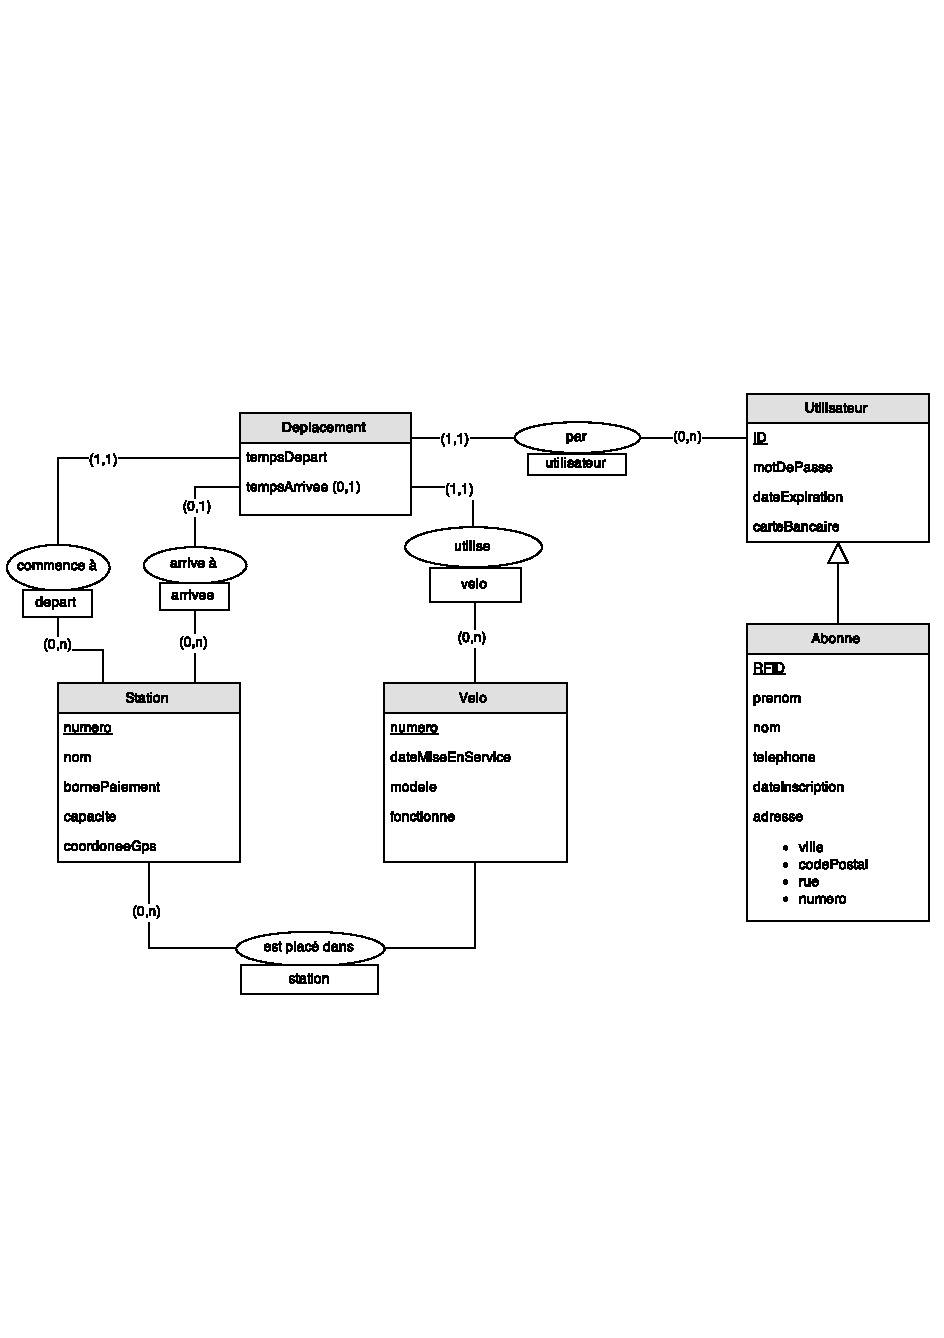
\includegraphics[scale=0.9]{entityassocdiagram.pdf}

\section*{Contraintes et hypothèses} %Contraintes

	\begin{itemize}
		\item Si un déplacement possède un temps d’arrivée, celui-ci doit être postérieur au temps de 			départ.
		
		\item Le temps de départ d’un déplacement doit être postérieur à la date de mise en service 			du vélo utilisé.
		
		\item Si l’utilisateur relié à un déplacement est un abonné, la date de départ doit être 				postérieur à sa date d’inscription.
		
		\item Les temps de départ et d’arrivée d’un déplacement doivent être antérieure à sa date 			d’expiration.
		
		\item La date d’inscription d’un abonné doit être antérieur à sa date d’expiration.
		
		\item Si un déplacement a un temps d’arrivée, il a une station d’arrivée et inversement.
		
		\item Un utilisateur ne peut être lié au maximum qu’à un seul déplacement sans date et 				station d’arrivée.
		
		\item Un vélo ne peut être lié au maximum qu’à un seul déplacement sans date et station 				d’arrivée.
		
		\item Si un vélo est lié à un déplacement sans date et station d’arrivée, il n’est placé dans 			aucune station.
		
		\item Si un vélo n’est lié à aucun déplacement sans date et station d’arrivée, il est placé dans 			la station d’arrivée de son dernier déplacement.
		
		\item Le nombre de vélo placé dans une station est inférieur ou égal à la capacité de celle-ci.
		
	\end{itemize}
	
	\subsection*{Remarque}
		Le type de généralisation n’est pas précisé car dans le cas d’une seule sous-entité, la 			généralisation est toujours partielle. La notion d’exclusivité ou de chevauchement n’a pas de 		sens dans ce cas.

\section*{Traduction relationnelle} %Relation
	
	\begin{itemize}
	
		\item Utilisateur(\underline{ID},motDePasse,dateExpiration,carteBancaire)
		
		\item Abonne( \underline{ID}, \underline{RFID}, prenom, nom, telephone, dateInscription, 				adresseVille, adresseCodePostal, adresseRue, adresseNumero)
		
		\begin{itemize}
			\item Abonne.ID référence Utilisateur.ID
		\end{itemize}
		
		\item Station(\underline{numero},nom,bornePaiement,capacite,coordonneeGps)
		
		\item Velo(\underline{numero},dateMiseEnService,modele,fonctionne,\textit{station})
		
		\begin{itemize}
			\item Velo.station référence Station.numero
		\end{itemize}
		
		\item Deplacement(\underline{utilisateur,tempsDepart},depart,velo,\textit{tempsArrivee},				\textit{arrivee})
		
		\begin{itemize}
			\item Deplacement.utilisateur référence Utilisateur.ID
			\item Deplacement.depart référence Station.numero
			\item Deplacement.velo référence Velo.numero
			\item Deplacement.arrivee référence Station.numero
		\end{itemize}
		
	\end{itemize}

\section*{Justification} % Justification

On a commencé par créer une table utilisateur pour stocker les données liées à ceux-ci.

Ensuite  on a hérité les abonnés des utilisateurs. On ajoute pas un héritage pour les utilisateurs temporaires, car toutes les données dont on a besoin pour ceux-ci sont déjà contenue dans la table Utilisateur.

On a aussi besoin d'une table station afin d'enregistrer les données les concernant.

On a ensuite ajouté la table vélo. Les vélos peuvent être lié à une station. Cela permet de savoir lequel est libre et lequel on peut donner à un utilisateur.

Pour terminer on ajoute une table déplacement pour permettre de sauvegarder l'historique de tous les déplacements effectués. Celle ci est liée à la table station pour connaitre l'endroit du départ et celui de l'arrivée. Elle est aussi lié à la table vélo pour savoir lequel est utilisé  et elle est aussi lié à la table utilisateur afin de savoir qui l'a effectué.

\end{document}